\documentclass[11pt,oneside]{article}
\input{coursHeadings}

\usepackage[%
    pdftitle={TD Communication technique},
    pdfauthor={Xavier Pessoles},
    colorlinks=true,
    linkcolor=blue,
    citecolor=magenta]{hyperref}



% \makeatletter \let\ps@plain\ps@empty \makeatother
%% DEBUT DU DOCUMENT
%% =================
\sloppy
\hyphenpenalty 10000

\newcommand{\Pointilles}[1][3]{%
\multido{}{#1}{\makebox[\linewidth]{\dotfill}\\[\parskip]
}}


\begin{document}


\newboolean{prof}
\setboolean{prof}{false}
%------------- En tetes et Pieds de Pages ------------
\pagestyle{fancy}
\renewcommand{\headrulewidth}{0pt}

\fancyhead{}
\fancyhead[L]{%
\begin{minipage}[c]{1.6cm}
\includegraphics[width=2cm]{png/logo_ptsi.png}%
\end{minipage}
\rule{2cm}{.5pt}
}

\fancyhead[C]{\rule{11cm}{.5pt}}

\fancyhead[R]{%
\begin{minipage}[c]{3cm}
\begin{flushright}
\footnotesize{\textit{\textsf{Sciences Industrielles\\ pour l'Ingénieur}}}%
\end{flushright}
\end{minipage}
}

\renewcommand{\footrulewidth}{0.2pt}

\fancyfoot[C]{\footnotesize{\bfseries \thepage}}
\fancyfoot[L]{\footnotesize{2011 -- 2012} \\ X. \textsc{Pessoles}}
\ifthenelse{\boolean{prof}}{%
\fancyfoot[R]{\footnotesize{TD -- CI 5 : Communication technique -- P}}
}{%
\fancyfoot[R]{\footnotesize{TD -- CI 5 : Communication technique}}
}


%\begin{center}
%\textit{Centre d'intérêt}
%\end{center}


\begin{center}
 \huge\textsc{CI 5 -- Communication technique}
\end{center}

\begin{center}
 \LARGE\textsc{Représentation des pièces mécaniques}
\end{center}

\vspace{.5cm}


\begin{contexte}
\begin{itemize}
\item Contexte technique : représentation de pièces issues du pilote automatique de voilier
\item Objectif : savoir passer d'une représentation 3D à une représentation 2D en respectant les normes de représentation.
\end{itemize}
\end{contexte}

\section*{Exercice 1 : Représentation de constituants du vérin du pilote automatique de voilier}

On s'intéresse au vérin d'un pilote automatique de voilier. La tige du vérin est reliée au safran du bateau et permet donc de modifier le cap du bateau. 

\begin{center}
\includegraphics[width=.9\textwidth]{png/fig1}
\end{center}

On donne un cahier des charges partiel associé à ce vérin.

\begin{minipage}[c]{.45\linewidth}
\begin{center}
\includegraphics[width=.9\textwidth]{png/fig2}
\end{center}
\end{minipage} \hfill
\begin{minipage}[c]{.45\linewidth}
\begin{center}
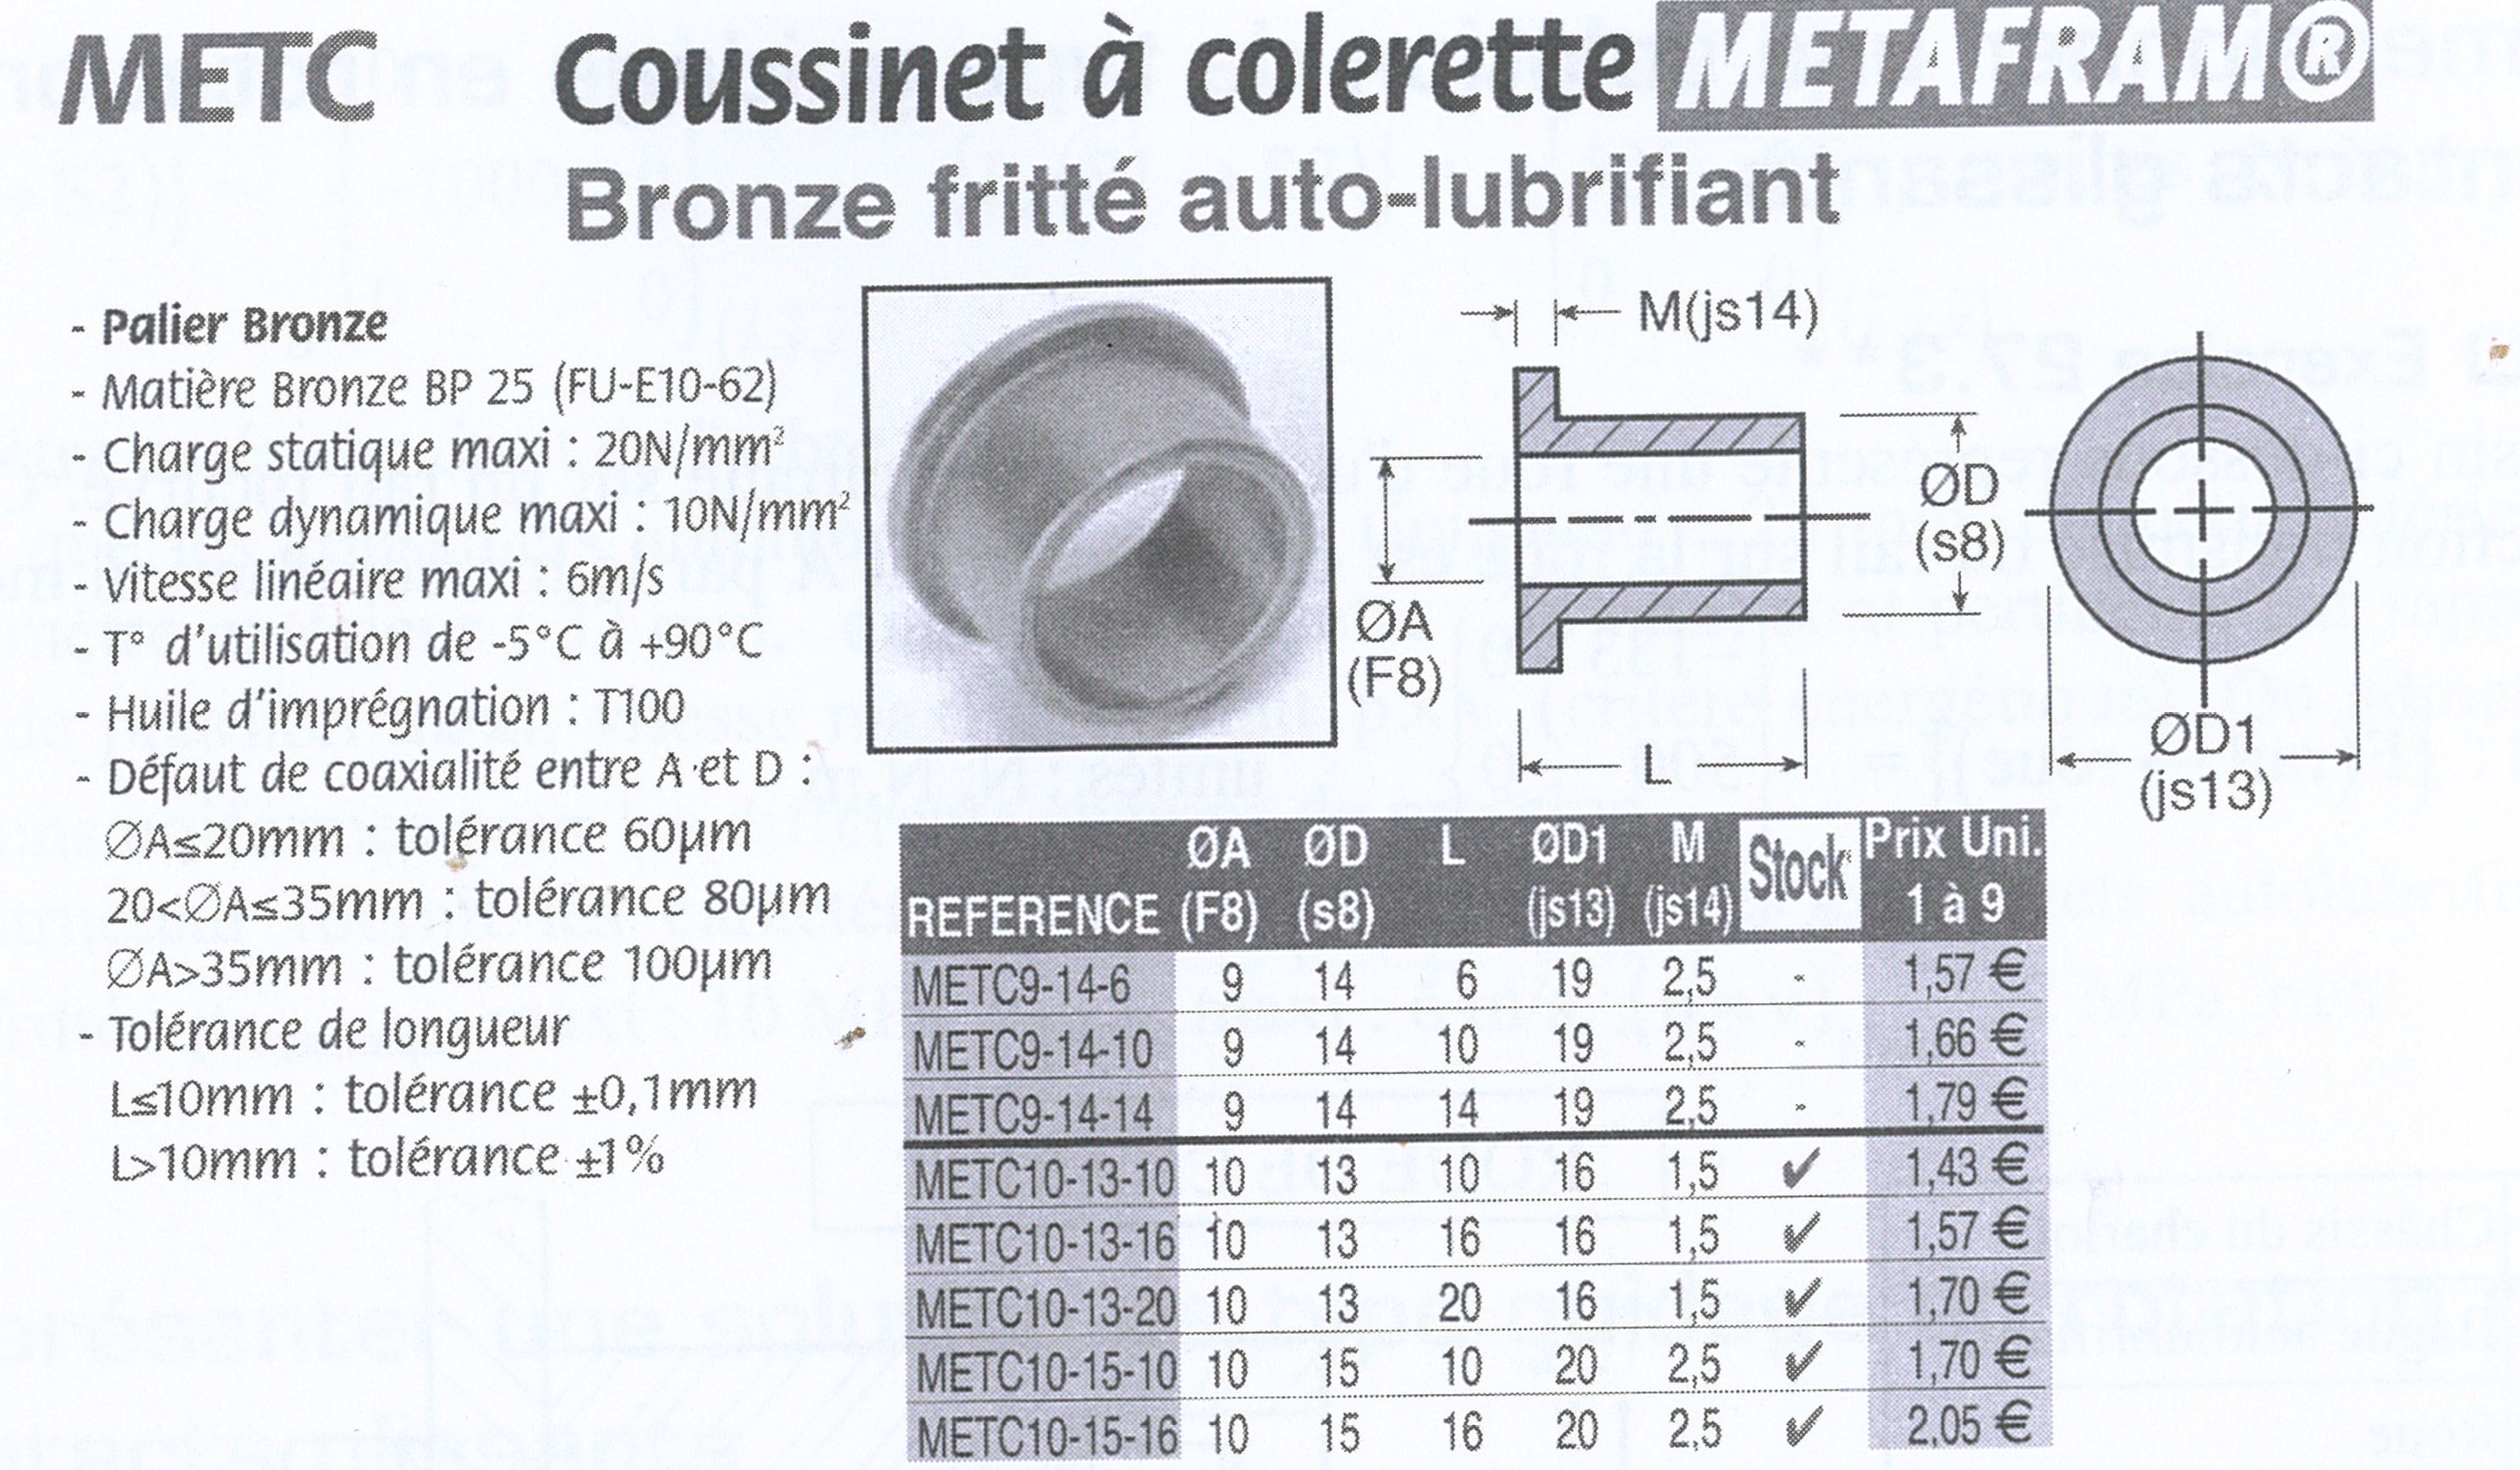
\includegraphics[width=.9\textwidth]{png/fig3}
\end{center}
\end{minipage} 

\paragraph{}
\textit{En utilisant les représentations 3D fournie, dessiner le nez de vérin en vue de face, de droite, de gauche, de dessus, de dessous et de derrière.}

\begin{center}
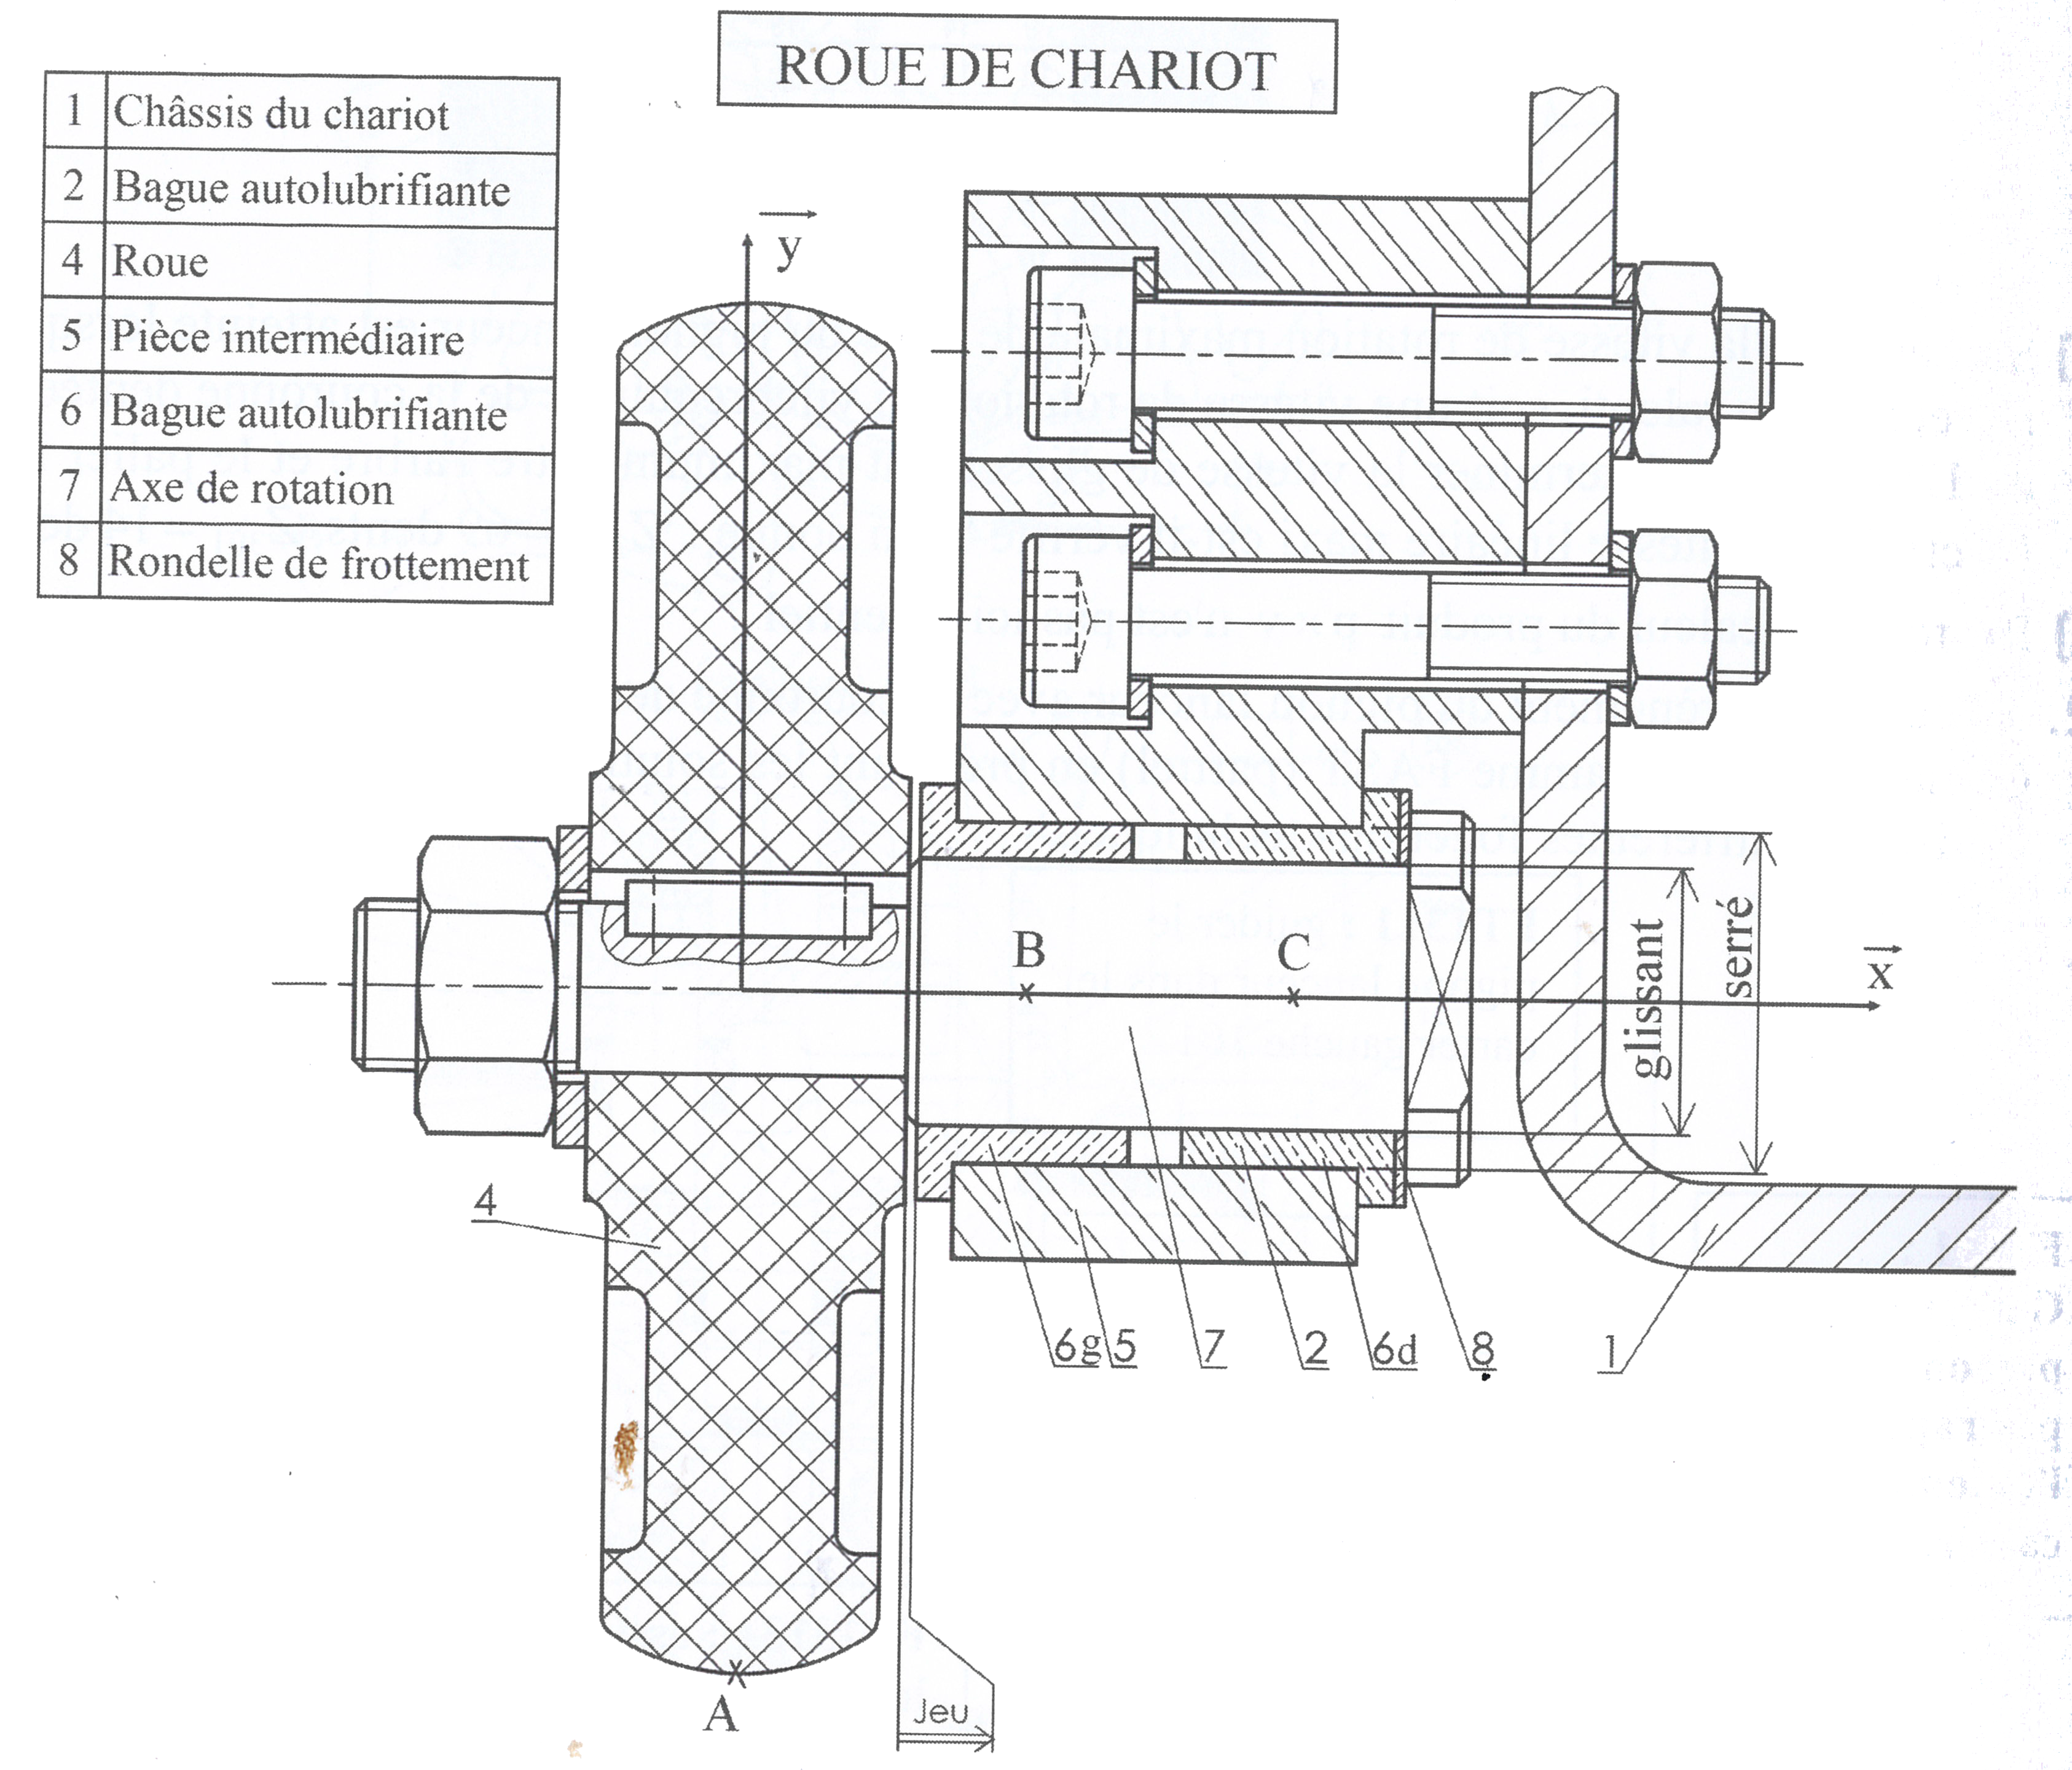
\includegraphics[width=.9\textwidth]{png/fig4}
\end{center}

\paragraph{}
\textit{Représenter une couple longitudinale du nez de vérin.}

\begin{center}
\includegraphics[width=16cm]{png/fig5}
\end{center}


\end{document}